

\chapter{Introdução à Genética Quantitativa}

A genética quantiativa, em suma, é o entendimento da relação entre fenótipo e genótipo. Para isto, é necessário estudar tudo que influência esta relção.

O modelo básico para um ambiente é F = G + A. Sendo F (Fenótipo), G (Genótipo) e A (Ambiente). Para que este modelo seja aplicado a vários ambientes, é necessário adicionar outro parâmetro GA que consiste na interação entre genótipo e ambiente. Como resultado temos F = G + A + GA.

A análise do fenótipo pode ser qualitativa, como é feita na genética mendeliana, ou quantiativa como será visto ao longo do texto.


\begin{table}[h]
\centering
\begin{tabular}{l l l}
\toprule
 Fator & \textbf{Caráter Qualitativo} & \textbf{Caráter Quantitativo}\\
\midrule
 \textbf{Controle Gênico} & Poucos & Poligênica \\
\textbf{Efeito Ambiental} & Nenhum ou Pouco & Alto \\
\textbf{Distribuição dos Dados} & Discreto (Classe) & Contínuo \\
\textbf{Estado do Caráter} & (P1xP2) e Qui Quadrado & Média e Variância \\
\textbf{Interação Alélica} & Dominância completa, incompleta e codominância &  Aditiva e Não Aditiva \\
\bottomrule
\end{tabular}
\caption{Caráter qualitativo x quantitativo} \label{tab:t01}
\end{table}


Os alelos são segmentos homólogos de DNA, os alelos dominantes, são representados por letras maiúsculas, enquanto os recessivos são representados por letras minúsculas. A Interação Alélica consiste na interação ou não de genes alélicos. 

As interações alélicas qualitativas são: dominância completa, dominância incompleta e codominância. As interações alélicas quantitativas podem se dividir em aditivas: quando cada alelo contribui individualmente para o valor genotípico e consequentemente para o valor fenotípico final; não aditivas: que podem ser dominância completa, parcial ou sobredominância.

A Epstasia não é uma interação alélica, consiste em uma interação gênica.

As interações de dominância criam uma perturbação na análise quantitativa do melhoramento genético.

\section{Interação Aditiva}

Para as demonstrações assuma dois genes A: A1,A2 e B: B1, B2. Além disso vamos adimitir valores para A1,B1,A2 e B2; sendo A1 = B1 = 30 unidades e A2 = B2 = 5 unidades.

Temos:

\begin{enumerate}
\item  Parental 1 (P1): A1A1B1B1 (120 unidades)
\item  Parental 2 (P2): A2A2B2B2 (20 unidades)
\item  *P1 e P2 são puros e contrastantes
\end{enumerate}

O cruzamento entre P1 e P2 terá como resultado F1 (A1A2B1B2), realizando a autofecundação em F1, teremos F2 que poderá gerar os genótipos como mostra a tabela abaixo:



\begin{table}[h]
\centering
\begin{tabular}{l l l}
\toprule
 \textbf{Genótipos} & \textbf{Frequência} & \textbf{Valor Genotípico}\\
\midrule
 A1A1B1B1 & 1/16 & 120 \\
 A1A1B1B2 & 2/16 & 95  \\
 A1A1B2B2 & 1/16 & 70  \\
 A1A2B1B1 & 2/16 & 95  \\
 A1A2B1B2 & 4/16 & 70  \\
 A1A2B2B2 & 2/16 & 45  \\
 A2A2B1B2 & 1/16 & 70  \\
 A2A2B1B1 & 2/16 & 45  \\
 A2A2B2B2 & 1/16 & 20  \\
\bottomrule
\end{tabular}
\caption{Genótipos Possíveis em F2} \label{tab:t01}
\end{table}

Considere \ol{X} como a média aritmética de um conjunto de valores.

A média pode ser calculada utlizando a soma simples ou a frequência dos itens.

\begin{equation}
\overline{X} =  \cfrac{\sum_{1}^{n} x_i}{n}
\end{equation}


\begin{equation}
\overline{X} = \cfrac{\sum_{1}^{n} f_i\times{x_i}}{f_i}
\end{equation}

Utilizando os dados da \ref{tab:t01}, pode-se calcular a média dos valores genotípicos de F2.


\begin{equation}
\overline{X} = \cfrac{\sum_{1}^{n} f_i\times{x_i}}{f_i}
\end{equation}

\begin{equation}
\overline{X} = \cfrac{
				1\times{120} + 
				2\times{95}  + 
				2\times{70}  + 
				2\times{95}  + 
				4\times{70}  +
				2\times{45}  + 
				1\times{70}  + 
				2\times{45}  + 
				1\times{20}
				}{16}
\end{equation}


\begin{equation}
\overline{X} = 70
\end{equation}


Quando a interação é aditiva, a médica de qualquer descendência é igual a média de seus pais. 

Segregantes transgressivos consistem em indivíduos em que seus valores genotípicos sejam maiores ou menores que seus pais. Para exemplificar, considere A1,B1,C1,D1 = 30 unidades e A2,B2,C2,D2 = 5 unidades. Considere os seguintes valores:

\begin{enumerate}
\item P1 = A1A1B1B1C2C2D2D2
\item P2 = A2A2B2B2C1C1D1D1
\item F1 = A1A2B1B2C1C1D1D2
\item F2 = Autofecundação de F1
\end{enumerate}

Dentre as 81 possibiblidades de F2, pode-se listar dois exemplos de segregantes transgressivos:

\begin{enumerate}
\item F2-1 = A1A1B1B1C1C1D1D1 = 240 unidades
\item F2-2 = A2A2B2B2C2C2D2D2 = 40
\end{enumerate}

\section{Interação de Dominância}

As interações de dominância ocorrem quando existe a relação de dominância entre alelos, ou seja, quando o alelo dominante está presente, o recessivo não contribui para a característica. Para exemplificar considere:

\begin{enumerate}
\item Gene A, sendo 'A' (Dominante) e 'a' (recessivo)
\item Gene B, sendo 'B' (Dominante) e 'b' (recessivo)
\item AA = 60 unidades
\item Aa = 60 unidades
\item aa = 10 unidades
\item BB = 60 unidades
\item Bb = 60 unidades
\item bb = 10 unidades
\end{enumerate}

Considere também os parentais P1:AABB (120 unidades) e P2:aabb (15 unidades). O cruzamento entre P1 e P2 dá origem ao descendente F1:AaBb (120). Neste caso, quando existe relação de dominância, o valor genotípico não será a média de seus parentais, podendo ser igual a um deles, como foi o caso.


\begin{table}[h]
\centering
\begin{tabular}{l l l}
\toprule
 \textbf{Genótipos} & \textbf{Frequência} & \textbf{Valor Genotípico}\\
\midrule
 AABB & 1/16 & 120 \\
 AABb & 2/16 & 120 \\
 AAbb & 1/16 & 70  \\
 AaBB & 2/16 & 120 \\
 AaBb & 4/16 & 120 \\
 Abbb & 2/16 & 70  \\
 aaBB & 1/16 & 70  \\
 aaBb & 2/16 & 70  \\
 aabb & 1/16 & 20  \\
\bottomrule
\end{tabular}
\caption{Genótipos Possíveis em F2} \label{tab:t03}
\end{table}

Com base nos dados da \ref{tab:t03} a média de F2 = 95, como a média de F1 é 120, pode-se concluir que houve a diminuição na média dos valores genotípicos. 

\begin{table}[H]
\centering
\begin{tabular}{l l l l l}
\toprule
 \textbf{X} & \textbf{AB} & \textbf{Ab} & \textbf{aB} & \textbf{ab} \\
\midrule
 \textbf{AB} & AABB & AABb & AaBB & AaBb \\
 \textbf{Ab} & AABb & AAbb & AaBb & Aabb \\
 \textbf{aB} & AaBB & AaBb & AaBB & aaBb \\
 \textbf{ab} & AaBb & Aabb & aaBb & aabb \\
 
\bottomrule
\end{tabular}
\caption{Genótipos Possíveis} \label{tab:t04}
\end{table}


\section{Grau médio de Dominância}

O grau médio de dominância mede a posição relativa do heterozigoto em relação à média dos homozigotos. 

\begin{figure}[h]
  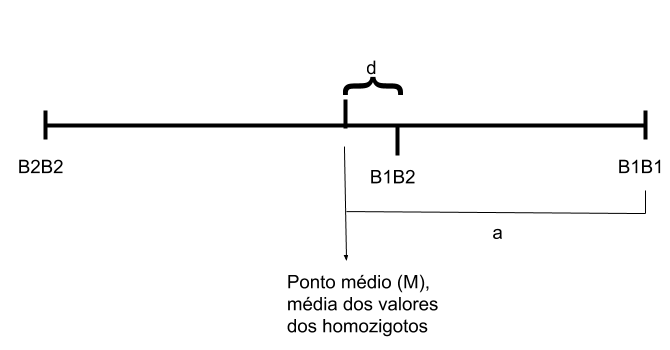
\includegraphics[width=0.9\linewidth]{img/grau-medio-dominancia.png}
  \caption{Grau Médio de Dominância}
  \label{fig:boat1}
\end{figure}


O valor do grau médio de dominância pode ser obtido dividindo-se d por a, esses valores são apresentados na \ref{fig:boat1}.


\begin{table}[H]
\centering
\begin{tabular}{l l }
\toprule
 \textbf{Resultado da Divisão} & \textbf{Interação Intra Alélica} \\
\midrule
 d/a = 0     & Interação  Aditiva  \\
 d/a = 1     & Dominância Completa \\
 0 < d/a < 1 & Dominância Parcial  \\
 d/a > 1     & Sobredominância     \\
\bottomrule
\end{tabular}
\caption{Genótipos Possíveis} \label{tab:t04}
\end{table}

O efeito de dominância mascara o processo de seleção, pois, ele dificulta o conhecimento dos indivíduos superiores pelos efeitos aditivos.

\section{Caráter Quantitativo}

O modelo para o estudo do caráter quantitativo é:

\begin{equation}
F = G + A
\end{equation}

Considere V(X) como a variância de X e Cov(X) como a covariância de X.

\begin{equation}
V(F) = V(G+A) \rightarrow V(F) = V(G) + V(A) + 2\times Cov(G+A)
\end{equation}

Como:

\begin{equation}
Cov(G+A) = 0
\end{equation}

Temos: 

\begin{equation}
V(F) = F(G+A) \rightarrow V(F) = V(G) + V(A) 
\end{equation}

A variância (V) é descrita pela seguinte fórmula: 

\begin{equation}
V(F) = \cfrac{\sum_{1}^{n} (x_i - \overline{X})^2}{n-1}
\end{equation}

ou

\begin{equation}
V(F) = \cfrac{\sum_{1}^{n} x^2 - [\sum_{1}^{n} x]^2}{n-1}
\end{equation}

\subsection{Dedução}

Para o cálculo da dedução da variância ambiental, considere um gene A, com dois alelos 'A' e 'a'.


\begin{table}[H]
\centering
\begin{tabular}{l l l l l}
\toprule
 \textbf{Genótipos} & \textbf{Nº Indivíduos} & \textbf{Frequência} & \textbf{Valor Genotípico} & \textbf{Val. Gen. Codificado} \\
\midrule
 AA & n1 & n1/n = D & X1 = u + a & a  \\
 Aa & n2 & n2/n = H & X2 = u + d & d  \\
 aa & n3 & n3/n = R & X3 = u - a & -a \\
\bottomrule
\end{tabular}
\caption{Dedução} \label{tab:t05}
\end{table}

Aplicando a fórmula da média na média genotípica:


\begin{definition}[Média Genotípica]
\begin{align}
&  Mg = \cfrac{\sum_{1}^{n} f_i\times{x_i}}{f_i} \\
&  Mg = D\times a + H\times d + R \times -a \\
&  Mg  = a \times (D-R) + H\times d \\
&  Mg = u + a\times(D-R) + H\times d
\end{align}
\end{definition}


\subsection{Variância Genética}

\begin{equation}
Va(x) = (\sum_{1}^{n} x_i^2) - (\sum_{1}^{n} f_i\times x_i)^2
\end{equation}

\begin{equation}
V(G) = D \times a^2 + H \times d^2 + R \times (-a)^2 - [a \times (D - R) + H \times d]^2
\end{equation}

\subsection{Estudo do Caráter}

Para o estudo do caráter, considere:

\begin{enumerate}
\item P1: AA
\item P2: aa
\item F1: Aa (P1xP2)
\item F2: [AA,Aa,aa]
\end{enumerate}


 
\begin{definition}[Análise de P1]

\begin{align}
&  Mg(P1) = u + a \times (D-R) + H \times d\\
&  Mg(P1) = u + a \times (1-0) + 0 \times d\\
&  Mg(P1) = u + a \\
\end{align}
\end{definition}

\begin{definition}[Variância de P1]

\begin{align}
&  V(P1) = D\times a^2 + H \times d^2 + R \times (-a)^2 - [ a \times (D-R) + H \times d ]^2 \\
&  V(P1) = 1\times a^2 + 0 \times d^2 + 0 \times (-a)^2 - [ a \times (1-0) + 0 \times d ]^2 \\
&  V(P1) = 1\times a^2 + -  1\times a^2 \\
&  V(P1) = 0
\end{align}

Portanto, como só existe um genótipo possível, não existe variância. A análise de P2 utiliza o mesmo método de P1, portanto, não há variância em P2.
\end{definition}


\begin{definition}[Análise de F2]

\begin{align}
&  Mg(F2) = u + a \times (\frac{1}{4}- \frac{1}{4}) + \frac{1}{2} \times d\\
&  Mg(F2) = u + \frac{1}{2} \times d\\
\end{align}
\end{definition}


\begin{definition}[Variância de F2]

\begin{align}
&  V(F2) = D\times a^2 + H \times d^2 + R \times (-a)^2 - [ a \times (D-R) + H \times d ]^2 \\
&  V(F2) = \frac{1}{4}\times a^2 + \frac{1}{2}\times d^2 + \frac{1}{4} \times (-a)^2 - [ a \times (\frac{1}{4}- \frac{1}{4}) + \frac{1}{2} \times d ]^2 \\
&  V(F2) = \frac{1}{4}\times a^2 + \frac{1}{2}\times d^2 + \frac{1}{4} \times (a)^2 - [ \frac{1}{2} \times d ]^2 \\
&  V(F2) = \frac{1}{2}\times a^2 + \frac{1}{2}\times d^2 - \frac{1}{4} \times d^2 \\
&  V(F2) = \frac{1}{2}\times a^2 + \frac{1}{4} \times d^2 \\
\end{align}
\end{definition}


\subsection{Variância Ambiental}

\begin{definition}[Fórmulas mais utilizadas]

\begin{align}
&  V(Amb) = V(P1) \\
&  V(Amb) = V(P2) \\
&  V(Amb) = V(F1) \\
&  V(Amb) = \frac{V(P1) + V(P2)}{2} \\
&  V(Amb) = \frac{V(P1) + V(P2) + V(F1)}{2} \\
&  V(Amb) = \frac{V(P1) + V(P2) + 2 \times V(F1)}{4} \\
\end{align}
\end{definition}
